\documentclass[11pt,a4wide]{article}
\usepackage{verbatim}
\usepackage{listings}
\usepackage{graphicx}
\usepackage{a4wide}
\usepackage{color}
\usepackage{amsmath}
\usepackage{amssymb}
\usepackage[dvips]{epsfig}
\usepackage[T1]{fontenc}
\usepackage{cite} % [2,3,4] --> [2--4]
\usepackage{shadow}
\usepackage{hyperref}
\usepackage{graphicx}
\usepackage[english]{babel}
\usepackage{float}
\usepackage{import}
\setcounter{tocdepth}{2}
\usepackage{listings}
\usepackage{color}
\usepackage{array}


\definecolor{blue}{rgb}{0,0,0.8}
\definecolor{mygray}{rgb}{0.5,0.5,0.5}
\definecolor{mymauve}{rgb}{0.58,0,0.82}

\lstdefinestyle{mystyle}
{ 
    backgroundcolor=\color{white},   
    commentstyle=\color{blue},
    keywordstyle=\color{magenta},
    numberstyle=\tiny\color{mygray},
    stringstyle=\color{mymauve},
    basicstyle=\footnotesize,
    frame=single,
    breakatwhitespace=false,         
    breaklines=true,                 
    captionpos=b,                    
    keepspaces=true,                 
    numbers=left,                    
    numbersep=5pt,                  
    showspaces=false,                
    showstringspaces=false,
    showtabs=false,                  
    tabsize=2, 
    stepnumber=2
}

\lstset{style=mystyle}


\begin{document}

\title{Solution to Radial Schr\"odinger in a 3D Harmonic Oscillator \break Computational Physics-Phy905 \break Project 2}
\author{Crispin Contreras}
\date{\today}
\maketitle


\begin{abstract}
This paper discusses the numerical solution for the radial Schr\"odinger equation in a 3D harmonic potential for two electrons. I consider the interaction and non-interaction of the electrons. I solved the equation with two different methods, the Jacobi method and the Armadillo eigenvalue solver. I compared the computational time for both methods and found that the Armadillo method is much faster than the Jacobi method. For the  non-interacting case we know the analytical solution and for the interacting case I compared to the values used in [2]. 
\end{abstract}



\section{Introduction}
We begin with the radial Schr\"odinger equation with a 3D harmonic oscillator potential. After some manipulation we get the equation to have less physical constants and also simplify it. The second derivative of the equation is approximated by the three point formula and we obtain a set of linear equations. We put them in matrix form which gives us the equation  $\ {\bf A}{\bf v} ={\bf \lambda}{\bf v}$. By writing it in this form we find that $\ {\bf A}$ is a tridiagonal matrix. This whole process is discussed in the Theory section. The Jacobi and Armadillo's eigenvalue solver are then used to solve for the eigenfunction $\ {\bf v}$ and eigenvalues. A discussion of how the Jacobi Algorithm works in given in the Methods section. Only the three lowest eigenfunctions and eigenvalues which are $\ {\bf \lambda} = 3,7,11$ were solved for. The precision of these values changed as the number of grid points (n) increased. Finally I discuss my results in the discussion section. 
\section{Theory}
\subsection{Single Electron}
We start with the radial part of the Schr\"odinger equation for one electron in a 3D harmonic oscillator. The general equation is
\[
  -\frac{\hbar^2}{2m} \left (\frac{1}{r^2} \frac{d}{dr} r^2 \frac{d}{dr} - \frac{l(l+1)}{r^2} \right)R(r) + V(r)R(r) = ER(r)
\]
In our case the potential $\ V(r)=\frac{1}{2}m\omega^2r^2$ and the energy is given by $\ E = \hbar\omega \left (2n + l + \frac{2}{3}\right)$ where $\ n=0,1,2,...$ and $\ l=0,1,2,...$ . Here $\ l$ is the orbital angular momentum of electron and n is the principal quantum number. The Schr\"odinger equation can be simplified by making the following substitution $\ R(r)=\frac{u(r)}{r}$ and we obtain 
\[
  -\frac{\hbar^2}{2m} \left (\frac{d^2}{dr^2} - \frac{l(l+1)}{r^2} \right)u(r) + V(r)u(r)= Eu(r)
\]
with the following boundary conditions $\ u(0)=0 \hspace{0.5cm} and  \hspace{0.5cm} u(\infty)=0$. In order to make the algorithm smoother I introduce a dimensionless variable $\ \rho=\frac{r}{\alpha}$ and obtain the modified Schr\"odinger equation 
\[
  -\frac{\hbar^2}{2m\alpha^2}\frac{d^2u(\rho)}{dr^2} + \left(\frac{\hbar^2}{2m\alpha^2}\frac{l(l+1)}{\rho^2} + V(\rho)        \right)u(\rho)= Eu(\rho)
\]
I only look at the solutions where $\l=0$ and plug in for the potential $\ V(\rho)=\frac{1}{2}k\alpha^2\rho^2$ and reach the form
\[
  -\frac{\hbar^2}{2m\alpha^2}\frac{d^2u(\rho)}{dr^2} +  \frac{1}{2}k\alpha^2\rho^2u(\rho)= Eu(\rho)
\]
We now multiply both side by $\ \frac{2m\alpha^2}{\hbar^2}$ and obtain 
\[
   -\frac{d^2u(\rho)}{dr^2} +  \frac{mk}{\hbar^2}k\alpha^4\rho^2u(\rho)=\frac{2m\alpha^2}{\hbar^2}Eu(\rho)
\]
The $\ \alpha$ constant can now be fixed so that 
\[
   \frac{mk\alpha^4}{\hbar^2}=1
\]
or 
\[
   \alpha=\left(\frac{\hbar^2}{mk}\right)^\frac{1}{4}
\]
I also define 
\[
	\lambda = \frac{2m\alpha^2}{\hbar^2}E
\]
I arrive at the final form for the equation 
\begin{equation}
   -\frac{d^2u(\rho)}{dr^2} + \rho^2u(\rho)=\lambda u(\rho)
\end{equation}
This equation is now easier to handle since it has less physical constants. In three dimensions the eigenvalues for $\ l=0$ are $\ {\lambda}_0 = 3, {\lambda}_1 = 7, {\lambda}_2= 11, ... $. 

I then use the three point formula for the second derivative 
\begin{equation}
  u''=\frac{u({\rho}_i+h) -2u(\rho) + u({\rho}_i+h)}{h^2} + \mathcal{O}(h^2)
\end{equation}
where h is our step. This is defined as 
\[
  h=\frac{{\rho}_max -{\rho}_min}{n+1}
\]
and the arbitrary value of $\ \rho$ is 
\[
	{\rho}_i = {\rho}_min + ih \hspace{0.5cm} i=0,1,2,..,n+1 
\]
the simplified Schr\"odinger equation now reads
\[
 - \left( \frac{u_{i+1}-2u_i +u_{i-1}}{h^2} \right) + {\rho}^2_iu_i = - \left( \frac{u_{i+1}-2u_i +u_{i-1}}{h^2} \right) + V_i u_i = \lambda u_i
\]
This equation can now be put in matrix form. The diagonal terms are given by $\ d_i = \frac{1}{h^2} + V_i $ and the non-diagonal terms are $\ e_i = -\frac{1}{h^2}$. 

\begin{equation}
\left(\begin{array}{ccccccc}
 	d_1& e_1& 0& \dots& \dots&  \dots &0\\
    e_1& d_2& e_1& 0& \dots& \dots &0 \\
    0& e_1 &d_3 & e_1 & 0 & \dots &0\\
    \dots& \dots   & \dots &\dots   &\dots & \dots &\dots\\
    \dots &\dots &\dots &\dots &\dots &\dots &\dots \\
    0 &\dots   &\dots  &\dots &e_1 &d_{n -1}& e_1 \\
    0 &\dots    &\dots  &\dots & 0  & e_1 & d_n \\
    \end{array} \right)   \left(\begin{array}{c}
    											u_1 \\
    											u_2 \\
    											\vdots \\ \vdots \\ \vdots \\ 
    											u_n
    			                \end{array}\right) = \lambda \left(\begin{array}{c}
    											u_1 \\
    											u_2 \\
    											\vdots \\ \vdots \\ \vdots \\ 
    											u_n
    			                \end{array}\right)        
\end{equation}
\subsection{Two Electrons with interaction}
We now consider two electrons in a harmonic oscillator potential. We start with the Schr\"odinger equation of the two electrons without interaction 
\[
	\left(-\frac{\hbar^2}{2m}\frac{d^2}{dr^2_1} -\frac{\hbar^2}{2m}\frac{d^2}{dr^2_2} + \frac{1}{2}kr^2_1 +\frac{1}{2}kr^2_2\right)u(r_1,r_2) = E^{(2)}u(r_1,r_2)
\]
where $\ u(r_1,r_2)$ is the wavefunction for the two electrons and $\ E^(2)$ is the respective energy. We know introduce a new set of coordinates which are $\ {\bf r }={\bf r_1 -r_2}$ and the center of mass coordinate $\ {\bf R}= \frac{1}{2}(r_1 +r_2)$. With some algebra I get that $\ {\bf r_1}={\bf \frac{r}{2} +R}$ and $\ {\bf r_2}={\bf R - \frac{r}{2}}$. Also the derivative 
\[
	\frac{d}{dr_1}= \frac{d}{dr}\frac{dr}{dr_1}+ \frac{d}{dR}\frac{dR}{dr_1}= \frac{d}{dr} +\frac{1}{2}\frac{d}{dR}
\]
and taking the derivative again we obtain the final form
\[
	\frac{d}{dr_1}\left(\frac{d}{dr_1}\right)=\frac{d^2}{dr^2} +\frac{1}{4}\frac{d^2}{dR^2} + \frac{1}{2}\frac{d}{dR}\frac{d}{dr} +\frac{1}{2}\frac{d}{dr}\frac{d}{dR}
\]
The same thing is obtain for $\ r_2 $ except that the cross terms are negative. Plugging this into the 2 electron Schr\"odinger equation we obtain
\[
	\left(-\frac{\hbar^2}{m}\frac{d^2}{dr^2} -\frac{\hbar^2}{4m}\frac{d^2}{dR^2} + \frac{1}{4}kr^2 + kR^2\right)u(r,R) = E^{(2)}u(r,R)
\]
Now we can separate the equations into $\ u(r,R)=\psi(r)\phi(R)$ doing this will give the energy as $\ E^{(2)} = E_r + E_R$ where 
$\ E_r$ is the relative energy and $\ E_R$ is the center of mass energy. We now introduce the Coulomb interaction between the electrons which is given by $\ V(r_1,r_2)= \frac{\beta e^2}{|{\bf r_1 -r_2|}}=\frac{\beta e^2}{r}$ where $\ \beta e^2=1.44eVnm$. Since this has the relative term r we can plug this into the equation. This means that we can ignore the center of mass equation for now. Plugging the Coulomb interaction I obtain 
\[
	\left(-\frac{\hbar^2}{m}\frac{d^2}{dr^2} +\frac{1}{4}kr^2 +\frac{\beta e^2}{r}\right)\psi(r) =E_r\psi(r)
\] 
we introduce the dimensionless variable $\ \rho=\frac{r}{\alpha}$ to get to the same form as equation (1). We then get
\begin{equation}
  \left(-\frac{d^2}{dr^2} + \frac{1}{4} \frac{mk}{\hbar^2} \alpha^4 \rho^2 + \frac{m \alpha \beta e^2}{\rho \hbar^2} \right)\psi (\rho)= \frac{m \alpha^2}{\hbar^2} E_r \psi(\rho)
\end{equation} 
we define a "frequency"
\[
	\omega_r = \frac{mk \alpha^2}{4 \hbar^2}
\]
and fix the $\ \alpha$ by requiring that 
\[
	\frac{m \alpha \beta e^2}{\hbar^2}=1
\]
or
\[
	\alpha =\frac{\hbar^2}{m \beta e^2}
\]
and 
\[
	\lambda = \frac{m\alpha^2}{\hbar^2}E_r
\]
Finally arrive at the final form
\begin{equation}
	\left(-\frac{d^2}{d\rho^2} + \omega^2_r \rho^2 + \frac{1}{\rho} \right) \psi(\rho) = \lambda \psi(\rho)
\end{equation}
We now treat $\ \omega_r $ as the strength of the potential and again consider only $\ l=0$. 

\section{Methods}
Two methods were implemented two solve the Schr\"odinger equation. One was the Jacobi method which consists of many similarity transformations and the other one was using Armadillo's eigenvalue solver which is called by $\ eig-sys$. I will discuss the Jacobi method here. I take much of the derivations from [1]. 
\subsection{Jacobi Method}
The Jacobi method consists of using many similarity transformation to reduce a matrix into diagonal form. In this case the matrix is $\ {\bf A}$. This method is chosen since doing a determinant for large matrices is impractical. The similarity transformation is defined by 
\[
	{\bf B} ={\bf S^{T}AS}
\]
The $\ {\bf S}$ has the following property $\ {\bf S^T}={\bf S^{-1}}$. In our case the similarity transformation is defined by 
\[
	s_{kk} =s_{ll}=cos(\theta), \hspace{0.3cm} s_{kl}=-s_{lk}=-sin(\theta), \hspace{0.3cm} s_{ii} =1 , \hspace{0.3cm} 
	 i \neq l \hspace{0.3cm} i \neq k
\]
the other terms are zero. The results for the $\ {\bf B}$ matrix are 
\begin{equation}
\begin{split}
 	b_{ik}=a_{ik}cos(\theta) -a_{il}sin(\theta), \hspace{0.3cm} i \neq k, \hspace{0.3cm} i \neq l \\
 	b_{il}=a_{il}cos(\theta)+a_{ik}sin(\theta), \hspace{0.3cm} i \neq k, \hspace{0.3cm} i \neq l \\
 	b_{kk}=a_{kk}cos^2(\theta) -2a_{kl}cos(\theta)sin(\theta) +a_{ll}sin^2(\theta), \hspace{0.3cm} \\
 	b_{ll}=a_{ll}cos^2(\theta)+2a_{kl}cos(\theta)sin(\theta) +a_{kk}sin^2(\theta), \hspace{0.3cm} \\
 	b_{kl}=(a_{kk} - a_{ll})cos(\theta)sin(\theta) +a_{kl}(cos^2(\theta) -sin^2(\theta))   \\
\end{split}
\end{equation}
The recipe is the to chose $\ \theta$ so that all non-diagonal elements $\ b_{kl}$ become zero. We require that $\ b_{kl}$ =$\ b_{lk}$ = 0 which then leads to 
\[
	b_{kl}=(a_{kk} - a_{ll})cos(\theta)sin(\theta) +a_{kl}(cos^2(\theta) -sin^2(\theta))=0	
\]
if $\ a_{kl}=0$ then this leads to $\ cos(\theta)$ = 1 and $\ sin(\theta)$ =0. To solve the equation above we define $\ tan(\theta)=t =\frac{s}{c}$ , $\ sin(\theta) =s$, $\ cos(\theta) = c$, and use the trigonometric identity $\ cos(2\theta)=\frac{1}{2(cot(\theta)-tan(\theta))}$ to obtain
\[
	cos(2\theta)=\tau= \frac{a_{ll} -a_{kk}}{2a_{kl}}
\]
using the trigonometric identity we obtain 
\[
	t^2 +2\tau t- 1=0
\]
resulting in 
\[
	t = -\tau \pm \sqrt{1+\tau^2}
\]
and we can obtain c and s by using trigonometric tricks 
\[
	c = \frac{1}{\sqrt{1+t^2}}
\]
and $\ s=tc $. In order to get the off-diagonal terms to be equal to zero or in our case  $\ \geq $ $\ 10^{-8}$ we have to complete many similarity transformations until this occurs. In order to figure this out we look at the Frobenius norm which is defined as 
\[
	||{\bf A}||_F = \sqrt{\sum_{i=1}^n \sum_{j=1}^n |a_{ij}|^2}
\]
One of the important properties of the Frobenius norm is that it's the same after similarity transformations. This property will be  used in the Jacobi algorithm. Solving the quadratic equation we find that $\ |\theta| \leq \frac{\pi}{4}$ having this property then leads to a minimization of the difference between $\ {\bf A}$ and $\ {\bf B}$ since 
\[
||{\bf B}-{\bf A}||_F^2=4(1-c)\sum_{i=1,i\ne k,l}^n(a_{ik}^2+a_{il}^2) +\frac{2a_{kl}^2}{c^2}.
\]
To summarize, the Jacobi methods consists of many similarity transformations in order to decrease the value of the off diagonal elements. This can be done by looking at the  norm. This algorithm was implemented in C++ and it's show below in listing 1. 

\lstinputlisting[language =C++,firstline=113, lastline=143, caption = This shows how the Jacobi method was implemented. The rotate function is called here and it's responsible for carrying out the operation in (6).]{"/home/quetzalcoatl/Computational_Physics_work/Project2/Code/Project2.cpp"}



\section{Results}
\subsection{Single Electron} 

The Jacobi algorithm was implemented in C++ according to section 3. This was then compared to the Armadillo's eigenvalue solver $\ eig-sys()$ to make sure it was working properly. The energy eigenvalues are know and were discussed in the theory sections. Their values 3,7,and 11 were used for calibration for getting the $\ \rho_{max}$. By trial and error we found that the best value for the three lowest states was $\ \rho_{max} = 5$. The results for the eigenvalues and computational times are shown in table 1 below. From table 1 we can see that as the value of n increases the eigenvalues get closer to the correct values. Table 1 also shows the number of iterations that the Jacobi method must make in order for the off-diagonal terms to be$\ \leq 10^{-8}$. From table 1 we can also estimate the number of similarity transformations in order to get the off-diagonal terms to $\ 10^{-8}$ which is roughly $\ 1.7n^2$. Finally we made a plot using matplolib for the corresponding three lowest state which is shown in figure 1. In this case we made sure the wavefunctions were normalized as $\ \int_0^\infty |u(\rho)|^2d\rho$. This was done by approximating the integral as a set of rectangles (like a histogram) and using the values of the normalized eigenfunctions as the height and the width from h we can calculate the area.The the integral is just 
\[
	\ \int_0^\infty |u(\rho)|^2d\rho \approx h\left(\sum_{j=1}^n |u_{j}|^2 \right)
\]
From this then we can get the normalized eigenfunctions by multiplying by $\ \frac{1}{h}$. This same procedure is done for the two electron case. 

\begin{figure}[H] 
\centering
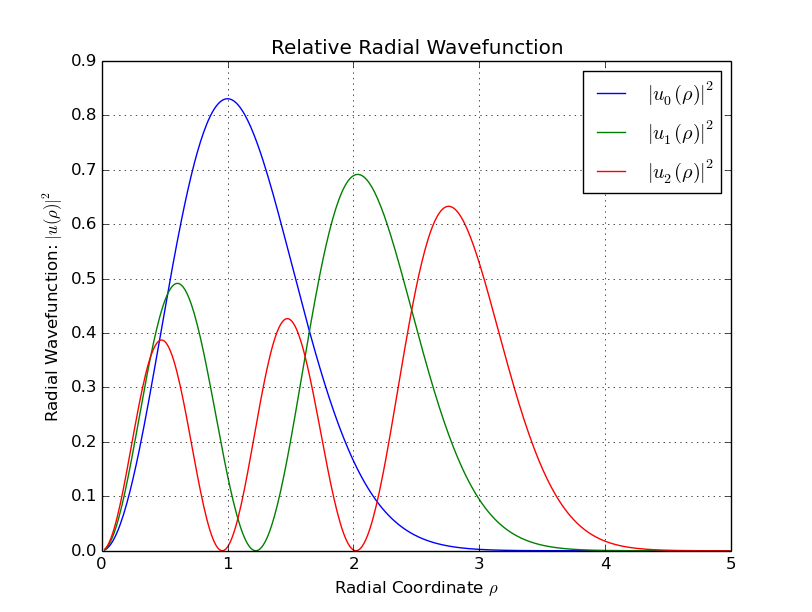
\includegraphics[width=100mm]{NI.png}
\caption{ Plot of the radial wavefunctions for the three lowest energies. The eigefunctions were normalized and we used $\ \rho_{max}$ = 5 and n=400.\label{overflow}}
\end{figure}
\begin{table}[H]
\centering
\label{my-label}
\begin{tabular}{| m{2cm} | m{3cm} | m{3cm} | m{3cm} | m{3cm} |}
 \cline{1-5}
  Grid Points, n&  3 Lowest Energy Eigenvalues For Jacobi, $\ \lambda$&  Calculation Time, $\ T_{Ja}$ [s]&   Calculation Time, $\ T_{arma}$ [s]& Number of iterations \\ \cline{1-5}
 50&  2.9969, 6.9850, 10.9634&  0.01653& 0.001274& 4040\\ \cline{1-5}
 100& 2.9992, 6.9962, 10.9908&  0.22181& 0.003996& 16475\\ \cline{1-5}
 200& 2.9998, 6.9990, 10,9978&  3.67701& 0.021410& 66828\\ \cline{1-5}
 300& 2.9999, 6.9996, 10.9991&  17.7895& 0.069452& 150798\\ \cline{1-5}
 350& 2.9999, 6.9997, 10.9994&  34.5932& 0.083118& 205757\\ \cline{1-5}
 400& 3.0000, 6.9998, 10.9996&  57.7010& 0.122340& 269021\\ \cline{1-5}
\end{tabular}
\caption{This table shows the number of grid points, the eigenvalues, Computational time, and the number of iterations. From here we can interpolate the number of similarity transformations needed to reach $\ 10^{-8}$.  }
\end{table}

\subsection{Two Interacting Electrons}
We use the same code for the single electron and modify it to include the Coulomb interaction. To see if the values are correct we use [2] and the values given by this source. This is shown in table 2.
\begin{figure}[H]
\centering
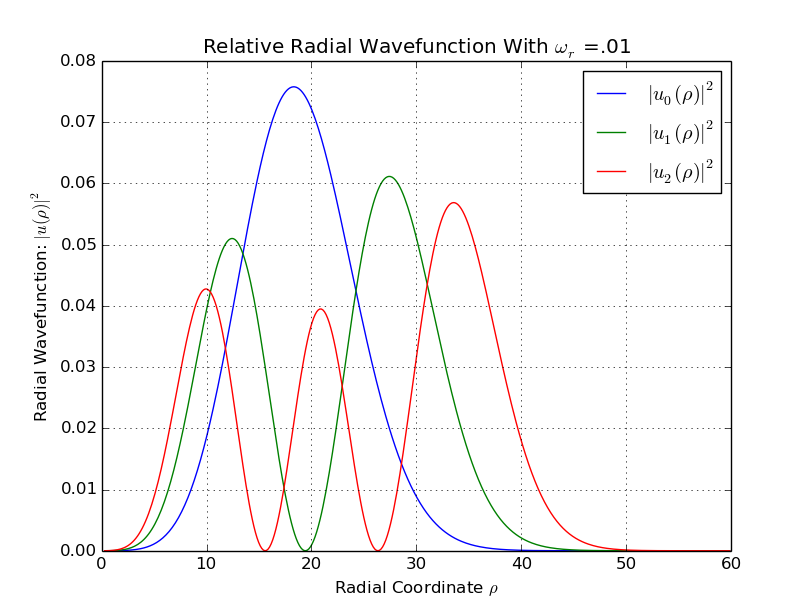
\includegraphics[width=100mm]{I_01.png}
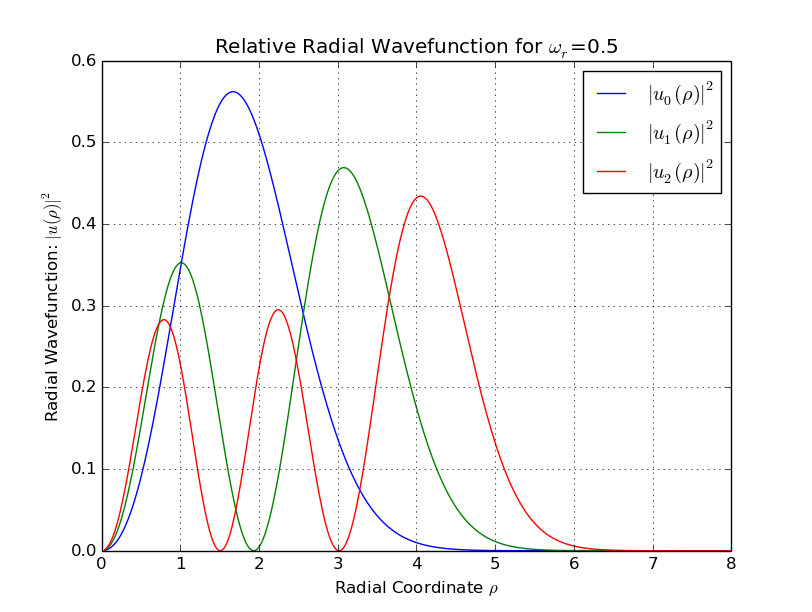
\includegraphics[width=100mm]{I_5.png}
\caption{This figure show the normalized eigenfunction for $\ \omega_r$ =0.01 and $\ \omega_r$=0.5. The values for $\ \rho_{max}$ are 60 and 8 repectively witn $\ n=400$. \label{overflow}}
\end{figure}
\begin{figure}[H]
\centering
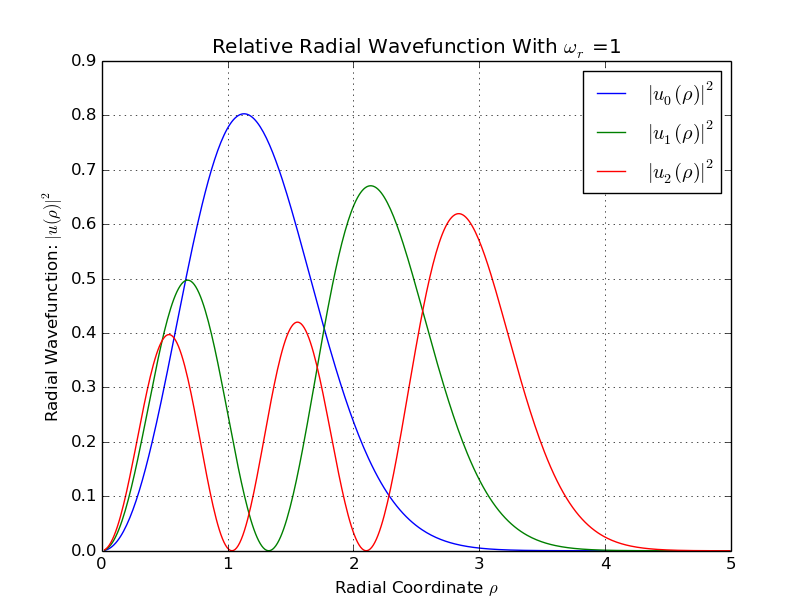
\includegraphics[width=100mm]{I_1.png}
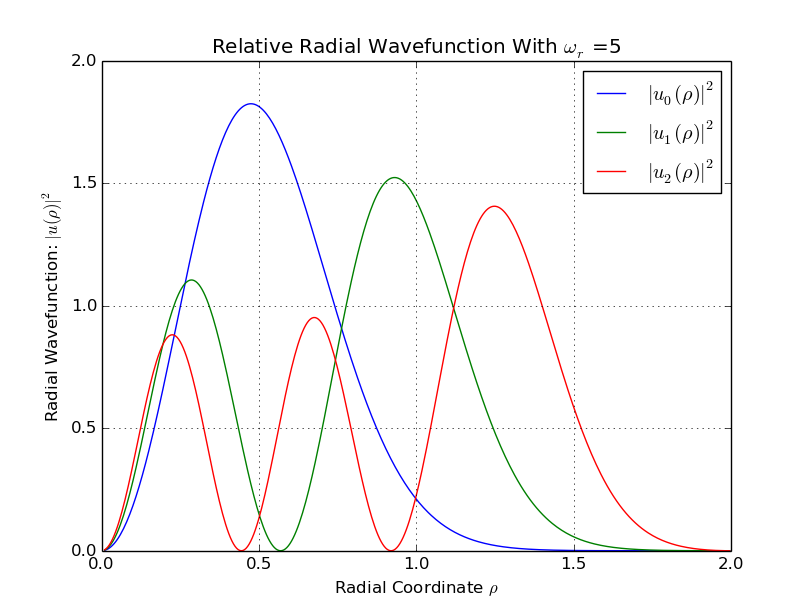
\includegraphics[width=100mm]{I_50.png}
\caption{This figure show the normalized eigenfunction for $\ \omega_r$ =1 and $\ \omega_r$=5. The values for $\ \rho_{max}$ are 8 and 2 repectively witn $\ n=400$. \label{overflow}}
\end{figure}

\begin{table}[H]
\centering
\label{my-label}
\begin{tabular}{| m{3cm} | m{3cm} | m{3cm} | m{3cm} |}
 \cline{1-4}
 Oscillator Frequency $\ \omega_r$&  Ground State Energy Eigenvalues, $\ \lambda$&  [2] Approximate Formula, 2$\ \epsilon'$&  [2]improved formula, 2$\ \epsilon'_int$ \\ \cline{1-4}
 0.01&  0.1058& 0.1050& --\\ \cline{1-4}
 0.05&  0.3500& 0.3431& 0.3500\\ \cline{1-4}
 0.25&  1.2500& 1.1830& 1.2500\\ \cline{1-4}
 0.5&  2.2300&  2.0566& --\\ \cline{1-4}
 1&  4.0578&    3.6219& --\\ \cline{1-4}
 5&  17.4485&   14.1863& --\\ \cline{1-4}
\end{tabular}
\caption{Values for the frequency $\ \omega_r$ and the energy eigenvalues. Also shown are the results from [2] which are the accepted values for the energies. We used these to make sure the algorithm was working correctly.}
\end{table}

\section{Discussion}
The implementation of the Jacobi algorithm produced good results as shown in table 1 since they have good agreement with the know energy values. From table 1 we obtain that approximately $\ 1.7n^2$ similarity transformations are needed to get the off-diagonal terms close to zero. This is less since our matrix is tridiagonal, for a full matrix a total of $\ 3n^2$ to $\ 5n^2$ transformations are needed[1]. We also saw that the Jacobi method has a very large computational time as opposed to the Armadillo's eigenvalue solver. 

In trying to get reasonable results the biggest problem with this algorithm was determining the value of n and $\ \rho_{max}$. This took some time since it was done by trial and error. Although when I figured out one of the values it was easier to determine the others by changing $\ \rho_{max}$ a bit. In order to start analyzing the interacting case we needed to use [2] to make sure the code was working correctly. For this I used the values for $\ \omega_r $=0.25 and 0.05 and compared to [2]. As shown in table 2 our results show that our program was working correctly. In addition to this I also checked that the norm of the lowest eigenvectors were equal to 1. This is because the Frobenius norm is no affected by transformations. Again my results shows that this was true. These were the "unit test" that I implemented to make sure my code was working correctly.

Finally I discuss the physics of plots. I use figure 1 as basis and compared to the other plots. The main result is that the eigenfunctions were stretch or squeezed depending on the size of $\ \omega_r$. For small values of $\ \omega_r$ we can see that eigenfunctions get stretched in the horizontal direction while for large values they get squeezed. We see that the electrons are further apart from each other when we include the interaction which is what is expected. 

\section{Conclusion}
The Jacobi algorithm was implemented and we found that it had a very large computational time compared to Armadillo's eigenvalue solver. Additionally it was a bit time consuming figuring out what the best value for $\ \rho_{max}$ was and similarly for n. The only way to do this was by trial and error. For the interacting case we found that the electrons get more spread out and this is what is expected since they have the same charges. The results for the interacting case were in agreement with [2] since the eigenvalues agreed. 

\section{References}
[1] M. Hjorth-Jensen.~Computational Physics, Lecture Notes Spring 2016.\break
[2] M.~Taut.Two electrons in an external oscillator potential: Particular analytical solutions of a coulomb correlation problem. Phys. Rev. A. 48, 3561-3566 (1993)

\section{Code Attachment}
\lstinputlisting[language =C++]{"/home/quetzalcoatl/Computational_Physics_work/Project2/Code/Project2.cpp"}

\end{document}

